\section{Trust Evaluation Metrics Based on The Supported Privacy Level}
\label{sec:blursense}
Privacy is part of trust evaluation.
The greater the level of privacy that an application or device can provide, the greater its trust evaluation would be.
A privacy enhancing system such as BlurSense~\cite{cappos2014blursense} can improve the trustworthiness of an Android device  
 by filtering or restricting the sensor data that an application can access.
In addition,
one can apply trust metrics to automate the application of Blursense itself.  For example, if an app has a low trust evaluation,
then BlurSense can restrict the sensor data that the app has access to.

\subsection{Motivation}
Although the sensing capabilities of smartphones enhance the convenience of user interfaces and
application usefulness, they also raise serious privacy
concerns~\cite{shabtai2010google}. For instance, through accessing sensor data,
malicious applications could retrieve sensitive information about the mobile
phone users, such as location, passwords, and credit card numbers~\cite{xu2012taplogger, 
miluzzo2012tapprints, xu2009stealthy, cai2011touchlogger}. They
even might be able to send sensitive information to remote
attackers~\cite{schlegel2011soundcomber, marquardt2011sp}. There
has been alarming news about privacy breaches of personal data on smart devices:
25\% of Android apps in Google Play can access user's personal
data~\cite{toomuch}; an iOS app can auto-post false piracy accusations on users'
Twitter accounts~\cite{tweetios}; apps could steal sensitive information like
passwords using the smartphone's motion sensors to determine key 
taps~\cite{xu2012taplogger}; and a huge botnet was discovered that was collecting sensor data
on more than a million end user smartphones~\cite{botnet}. The
Federal Trade Commission (FTC) even recommended that mobile platforms should
provide in-time disclosures to users of accessing sensitive content on smart
devices~\cite{ftc}. 

\subsection{Applying Trust Metrics to BlurSense}
Trust metrics can also be used by privacy enhancing tools such as BlurSense to limit access to sensor data.
The current access control to the smartphone resources,
such as sensor data, is static and coarse-grained. 
%However, such defense is pre-determined by the manufacturer. 
Take the
Android platform as an example, the access permissions are
either granted or denied completely during the installation of
applications based on a request XML manifest file. As a result,
applications may ask for more permissions than are actually
required for operation. Having been granted the requested
permissions, applications have access to those resources permanently. 
A trust metric could be used during installation of an app to decide whether or not
to deny access specified in its manifest file.  
A better approach is to restrict access to sensor data in a
dynamic and fine-grained framework.
Some systems that have been proposed to address this
issue require modifications to the Android
platform~\cite{conti2011crepe, hornyack2011these}. This increases the cost of maintenance, is
less flexible and cannot be used in legacy systems. In addition,
the user would need to trust that the new operating system is
not malicious and is not more vulnerable than the standard one.

\begin{figure}%[htd]
  \centering
  % Requires \usepackage{graphicx}
  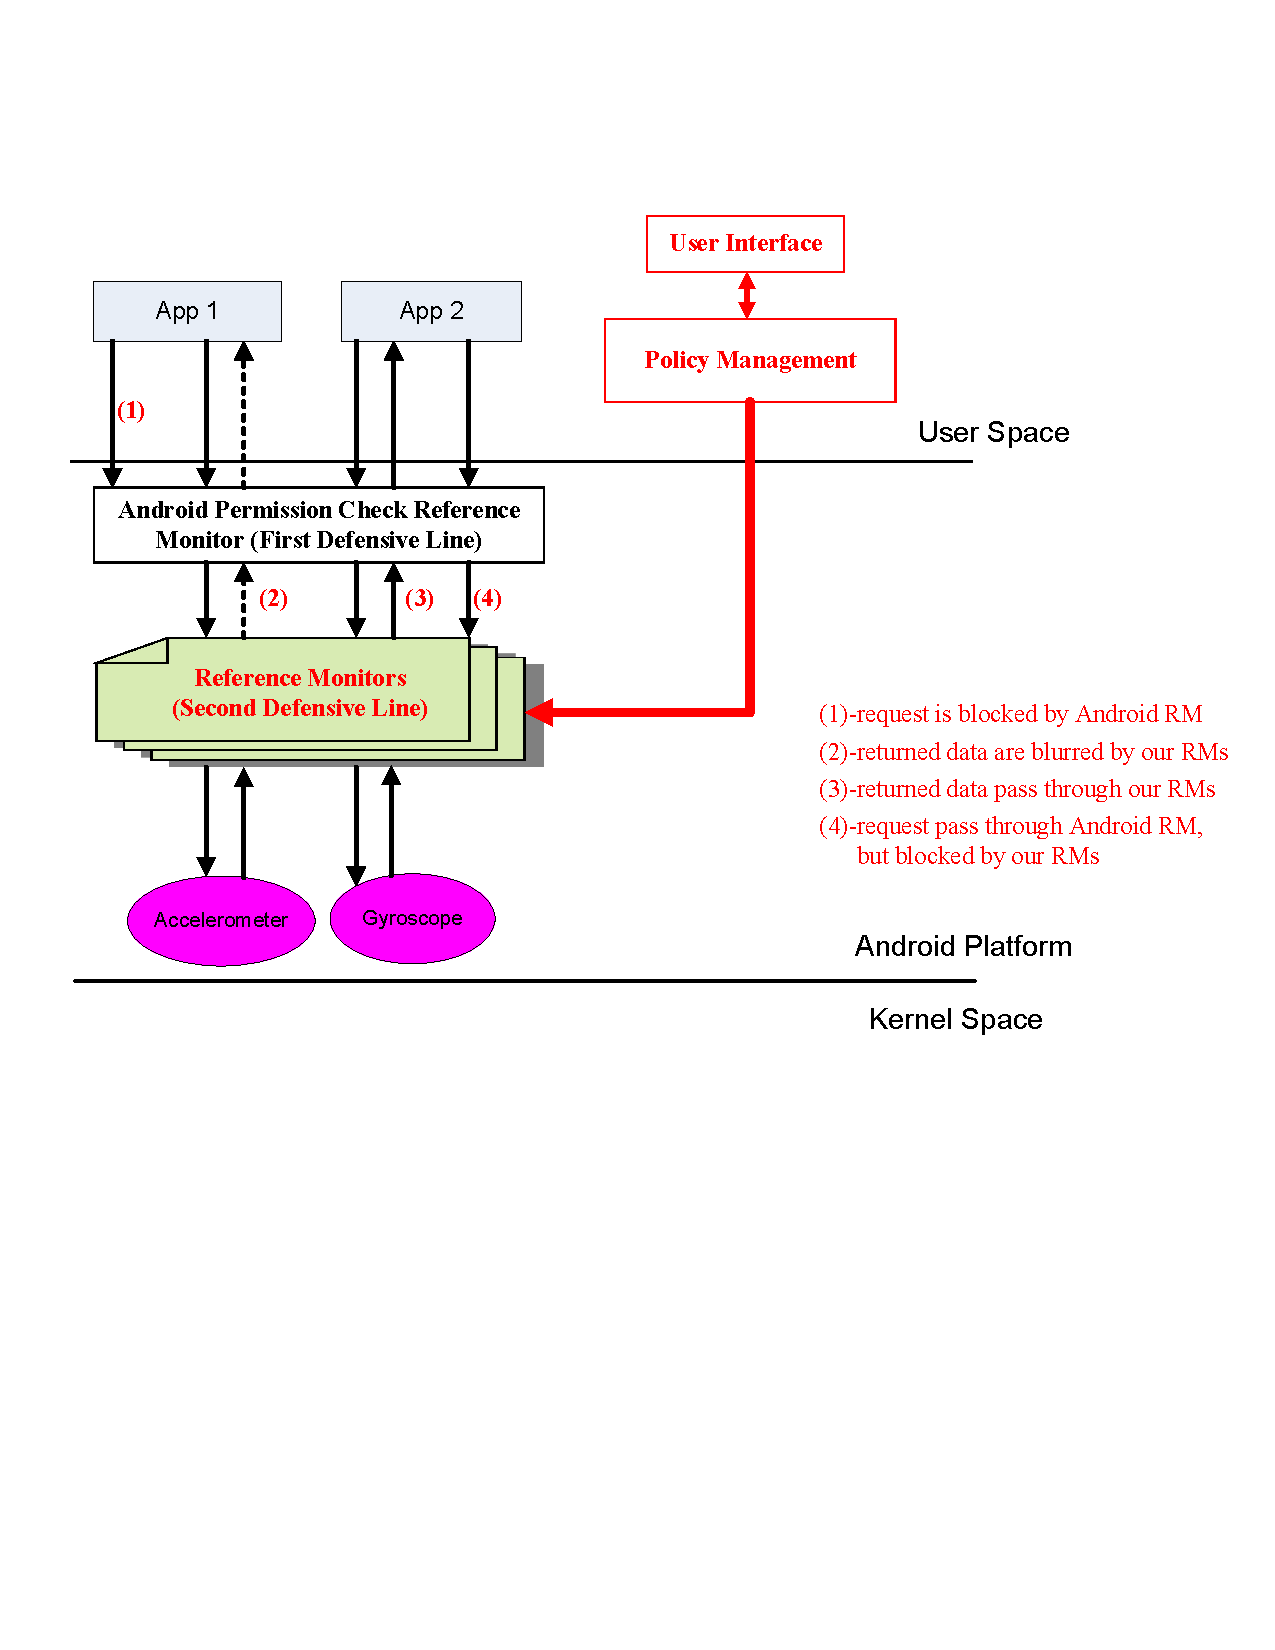
\includegraphics[width=3.7in]{refMonDesign.pdf}\\
  \caption{System architecture based on reference monitors.}
  \label{Fig:design}
\end{figure}

The BlurSense project deals with this problem of fine-grained conrol of sensor data
by requiring that all untrusted apps be installed
through an app that filters sensor data through a reference monitor~\cite{cappos2014blursense}, 
as shown in Figure~\ref{Fig:design}.
The policy for filtering can be set by the user based on a trust metric.
 The reference
monitor can exercise fine-grained control to degrade the accuracy of the sensor data, render it 
completely meaningless, or pass it through unchanged.  
In the case of geolocation, GPS measurements can be set to the center of the nearest
large city or random noise can be added.  Another approach would be to allow the user to decide
whether to install the app or not, based on the trust evaluation. 
%based on the sensor data requested in the manifest file.
The reference monitor approach poses less risk than others; the worst that can happen is
that the app will have the same access to the sensor data that
is permitted by the manifest file. In the best case, BlurSense
would limit the access to sensor data based on a combination of trust metrics for the app.
BlurSense is currently able to filter data on battery level, CPU usage, geolocation (latitude, longitude,
altitude, accuracy, and speed if available), and network related measurements
such as mobile network type and operator, nearby WiFi access point
and Bluetooth devices.

\eat{
Currently, implemented sensor modules and
the available contextual information are classified into three
categories: device specific (percentage of battery power level,
CPU and memory utility), location related (latitude, longitude,
altitude, accuracy, and speed if available), and network related
(mobile network type and operator, nearby WiFi access point
and Bluetooth devices). While sensor modules are the system
hooks with read access to valuable sensor resources, they
cannot manipulate sensor data. Additionally, the sensor API
also provides a base registry service with a common interface
for use by a sensor implementation. } % end comment
\eat{For both local and remote
processes to access sensor data, a JSON/sl4a library
is incorporated to provide data in an unified format. In case
newer sensors appear on future mobile devices, developers can
add newly implemented sensors into this framework rather
easily. 
%The registry service listens for connection on a set of predefined ports via XML-RPC. 
Thus, both local and remote
process can connect to these ports and register for sensor
updates.
Our preliminary work in this area has resulted in working 
code~\cite{seattle-sensor-git}, tutorials~\cite{seattle-sensor-project}, and a 
blog for problem discussion~\cite{sensor}. Several different groups have
already used our early-stage proof-of-concept to solve problems across a variety
of domains, demonstrating the potential of sharing sensor data. 
} % end comment
